% !TeX root = ../../thesis.tex
\chapter{Applications: Mechanical integrity of infilled structures}\label{ch:infill}

\section{Introduction}

Biodegradable metallic materials are gaining more attention as promising candidates for bone implants in the recent decade. For tissue engineering applications, these biodegradable materials are magnesium (Mg), zinc (Zn), and iron (Fe), each of which has its own positive and negative features. They have been widely used in orthopedics and cardiovascular applications, both in commercially pure (CP) and alloyed form. They possess acceptable biocompatibility and bioabsorption properties, as well as sufficient mechanical stability. 

Among these biodegradable metallic materials, Mg is gaining interest for use in bone repair applications. Despite its high degradation rate, pure Mg and Mg alloys have similar physical and mechanical properties as the natural bone, making them a perfect choice to prevent stress shielding, which is the one of the main causes of implant failure. For this reason, Mg-based alloys are called revolutionary metals in biomedical applications \cite{Shuai2019}. 

In order to take advantage of these materials in bone tissue engineering applications, their degradation parameters should be tuned to the rate of regeneration of the bone. One approach for investigating biodegradation behavior is to construct computational models to assess the biodegradation properties prior to conducting any in-vitro or in-vivo tests. In addition to degradation tuning, these models can be used for evaluating the mechanical integrity of the implants, which can be considered as an important application in bone tissue engineering. 

Mechanical integrity can be studied via the change of mechanical properties of the implant over time, an example of which is the stiffness variations of the implant while the degradation takes place. In this study, the change of stiffness of porous structures during the biodegradation process is investigated by coupling the degradation model and a mechanical analysis model. Such coupling allows studying the correlation of variations in different quantities in both models, such as the effect on mass loss on the compliance of the structure and as a result, on the stiffness. 

The infilled structures are opted due to their interesting properties to be used in biomedical applications, one of which is to allow more interaction between the implant and the body environment \cite{Birmingham2012}. A bone implant with a proper lattice structure manufactured with functionally graded materials can improve the healing process of bone defects \cite{Mahmoud2017}. In the current study, the investigated infilled structures are created using a topology optimization (TO) routine, in which a set of different volume constraints leads to different final shapes. 

Performing TO on degrading structures has been rarely studied, the reason of which is the difficulty of evaluating the sensitivity of the optimization models in presence of complex biodegradation mechanisms. Zhang et al. \cite{Zhang2021} presented such a model for a simplified degradation mechanism in which a constant mass loss from the surface was considered in a sophisticated level-set based TO to mimic the biodegradation process. In their later work \cite{Zhang2021a}, they enhanced their implementation from the TO perspective by extending and verifying it in the microscopic scale for stiffness changeable composite structures. Despite the technical difficulty, the presented model in the current study can be a first step towards building a coupled model for designing implants with optimizing the structure while the biodegradable tuning is taken into account. In this model, the change in the compliance of the degrading structure is calculated in each step of degradation, making it possible to use it later as the objective function of the TO process so as to consider the effect of the biodegradation process.


\section{Methods}

This section provides the mathematical and physical frames for the topology optimization of feature-rich structures based on the reaction-diffusion equation-driven (RDE-driven) level-set method. In section \ref{Section: level-set-based topology optimization method}, the basic concept of the RDE-driven TO method is introduced. In section \ref{Section: Maximum length-scale constraint}, the local volume constraint is introduced in this workflow. The key idea here is to use a variational method (PDE-filter) to compute such local volume fraction which does not require the explicit knowledge of the spatial information of the neighboring elements. The optimum design problem is formulated in section \ref{Section: topology optimization problem}. Finally, we present several two-dimensional test cases in section \ref{Section: numerical examples}.


\subsection{Level-set-based topology optimization method}\label{Section: level-set-based topology optimization method}
First, the basic concept of the level-set-based TO method is introduced. We follow the lead of Yamada et al.\ \cite{yamada2010topology}. A structural topology optimization problem can be replaced by an optimum design problem to find the optimal material distribution. In other words, this technique is essentially to answer the question that ‘‘where should the material be placed?'' or ‘‘where should the hole be nucleated?''. Let the computational domain be denoted as $\Omega \subset \mathbb{R}^d$, where $d=2$. A solid subdomain is then defined as $\Omega_{s} \subseteq \Omega$ and a void domain is  as the complementary domain $\Omega \backslash \Omega_{s}$. An implicit level-set function $\phi \left(\boldsymbol{x}\right)$ is introduced and it can be defined to have a piecewise profile as
\begin{equation}
	\left\{\begin{array}{ll}
		{0<\phi(\boldsymbol{x}) \leq 1} & {\text { for } \boldsymbol{x} \in \Omega_{s} \backslash \partial \Omega_{s}} \\
		{\phi(\boldsymbol{x})=0} & {\text { for } \boldsymbol{x} \in \partial \Omega_{s}} \\
		{-1 \leq \phi(\boldsymbol{x})<0} & {\text { for } \boldsymbol{x} \in \Omega \backslash \Omega_{s}}.
	\end{array}\right.
\end{equation}
Therefore, the solid--void interface $\partial \Omega_{s}$ can be represented by the zero level-set iso-surface.  

Next, using a Heaviside step function, the material field can be modeled using a ‘‘1/0 binary structure'' by the projection of the level-set function $\phi(\mathbf{x})$ to the characteristic function $\chi_{\phi}$ as
\begin{equation}
	\chi_{\phi} :=\left\{\begin{array}{ll}
		{1} & {\text { for } \phi\left( \boldsymbol{x} \right) \geq 0} \\
		{0} & {\text { for } \phi\left( \boldsymbol{x} \right)<0}.
		\label{eq: characteristic function}
	\end{array}\right.
\end{equation}
Using the Ersatz material approach, the material properties inside the computational domain $\Omega$ can be expanded using the obtained $\chi_{\phi}$. The level-set function is evolved as the solution of a reaction--diffusion equation, which can be semi-discretized in a fictitious time-step $\Delta t$, as follows:
\begin{equation}
	\left\{\begin{array}{ll}
		\dfrac{1}{\Delta t} \left( \phi_{n+1} - \phi_{n} \right) =- \left( \tilde{C} \mathcal{F}' -\tau \nabla^{2} \phi_{n+1} \right) & \text{in }\Omega\\
		\nabla \phi \cdot \boldsymbol{n} = 0 & \text{on } \partial\Omega \\
	\end{array}\right.
	\label{eq: reaction diffusion equation semi discretize}
\end{equation}
where $\boldsymbol{n}$ is the unit normal vector, $\mathcal{F}'$ is the topological design sensitivity, $\tilde{C}$ is the normalizer for the sensitivity, and $\tau$ is the regularization parameter, which can be used to control the complexity of the optimal configuration. The subscript $n$ indicates the fictitious time step. For more details, the reader are referred to in the case studies in our previous work\ \cite{li2021full}. 

\subsection{Maximum length-scale constraint}\label{Section: Maximum length-scale constraint}
To generate some feature-rich structures observed in the natural system, e.g., bone structure, a geometrical constraint is introduced. Here, we adopt the idea of Wu et al.\ \cite{wu2017infill} by imposing a maximum allowable volume fraction to the local averaged value of the characteristic function, $\bar{\chi}$. To approximate the maximum value of $\bar{\chi}_i$, we use the $p$-norm function as
\begin{equation}
\max_{\forall i} \left(\bar{\chi}_i \right) \approx  
\|\bar{\chi}_i \|_{p}=\left(\sum_i^n \bar{\chi}_{i}^{p}\right)^{1/p}
\leq \left( \sum_{i}^n \bar{V}_{\max}^p \right)^{1/p}, 
\end{equation}
and it can be rewritten as
\begin{equation}
\left(\dfrac{1}{n} \sum_{i} \bar{\chi}_{i}^{p}\right)^{1 / p} \leq \bar{V}_{\max },
\end{equation}
where $n$ is the total number of vertices. Note that in FreeFEM\ \cite{Hecht2012}, the design variable--characteristic function is defined on the nodes of each element. $ \bar{V}_{\max }$ is the maximum allowable local volume fraction. We set $p=10$ in this paper. 

We use a PDE-filter\ \cite{lazarov2011filters,kawamoto2011heaviside} to compute the local average value $\bar{\chi}$, as
\begin{equation}
	\left\{\begin{aligned}	
		& -r^2 \nabla^2 \bar{\chi} +  \bar{\chi} =  \chi & \text{ in } \Omega \\
		& \nabla \bar{\chi} \cdot \boldsymbol{n} = 0 & \text{ on } \partial \Omega,
	\end{aligned}\right.
	\label{Eq: pde filter}
\end{equation}
where $r$ is the filter radius. 

\subsection{Optimum design problem for feature-rich structures}\label{Section: topology optimization problem}

The underlying physics is the linear elasticity where the following assumptions are made: (1) small displacements and deformations are observed (linear elasticity), and (2) the body-force and gravity are neglected. Furthermore, the context of interest here is to minimize the mean compliance of the structure, or in other words, to maximize the stiffness of the structure. Therefore, the topology optimization problem can be formulated as
\begin{subequations}
	\begin{equation}
		\inf _{\chi_{\phi} \in \mathcal{X}} J(\Omega)=\int_{\partial \Omega_{s}^{N}} \boldsymbol{t} \cdot \boldsymbol{u} d \Gamma,
		\label{eq: objective function}
	\end{equation}
	\begin{equation}
		\text { s.t. }\left\{\begin{array}{ll}
			-\operatorname{div}(\mathbb{C}_{\chi_{\phi}} : e(\boldsymbol{u}))=0 & \text { in } \Omega \\
			\boldsymbol{u}=\boldsymbol{u}_{0} & \text { on } \partial \Omega^{D} \\
			(\mathbb{C}: e(\boldsymbol{u})) \cdot \boldsymbol{n}_{s}=\mathbf{t} & \text { on } \partial \Omega^{N} \\
			G_{1}=\dfrac{\int_{D} \chi d \Omega}{\int_{D} d \Omega}-V_{\max } \leq 0 & \\
			G_2=\left(\dfrac{1}{n} \sum \bar{\chi}^{p}\right)^{1 / p}-\bar{V}_{\max } \leq 0 & \\
			-r^2 \nabla^2 \bar{\chi} +  \bar{\chi} =  \chi & \text{ in } \Omega \\
			\nabla \bar{\chi} \cdot \boldsymbol{n} = 0 & \text{ on } \partial \Omega,
		\end{array}\right.
		\label{eq: governing equation and constraints}
	\end{equation}
	\label{eq: topology optimization mathematical model}
\end{subequations}
where $\mathbb{C}$ is the fourth-order elasticity tensor, $\boldsymbol{t}$ is the surface traction, and $e\left(\boldsymbol{u}\right)$ is the linearized strain tensor. Using the characteristic function $\chi_{\phi}$, the elasticity tensor $\mathbb{C}$ can be expanded as
\begin{equation}
	\mathbb{C}_{\chi_{\phi}} = \chi_{\phi} \left(\mathbb{C}_{\text{s}} - \mathbb{C}_{\text{v}} \right) + \mathbb{C}_{\text{v}},
\end{equation}
where $\mathbb{C}_{\text{s}}$ and $\mathbb{C}_{\text{v}}$ are the constitutive tensors for solid and void (weak) materials, respectively. 

As it is well-known that the mean compliance problem is self-adjoint. Therefore, the topological design sensitivity can be derived as
\begin{equation}
	\mathcal{F}^{\prime}=-\left(e(\boldsymbol{u}): \mathbb{C}_{\chi_{\phi}}\right): e(\boldsymbol{u})+\lambda_{1} + \lambda_2 \mathcal{G}',
	\label{Eq: design sensitivity}
\end{equation}
where $\lambda_{1}$ and $\lambda_{2}$ are the Lagrange multipliers associated to the global and local averaging volume constraints, respectively. They can be updated using the augmented Lagrange method\ \cite{li2021full}.

The sensitivity associated to the local volume constraint $\mathcal{G}'$ computed as the solution of the following system of equations:
\begin{equation}
	\left\{\begin{aligned}	
		& -r^2 \nabla^2 \mathcal{G}' +  \mathcal{G}' =  \dfrac{\partial G_2}{\partial \bar{\chi}} & \text{ in } \Omega \\
		& \nabla\mathcal{G}' \cdot \boldsymbol{n} = 0 & \text{ on } \partial \Omega.
	\end{aligned}\right.
	\label{Eq: G'}
\end{equation}

\subsection{Numerical examples}\label{Section: numerical examples}
A two-dimensional test case is presented hereinafter. The computational domain is a rectangle with its dimension of $2.5L \times 1.0L$. There are two holes inside the domain. The surface traction $\boldsymbol{t}=\left[0,-1\right]^{\operatorname{T}}$ is distributed evenly on the boundary of the right-hand side hole, and that of the left-hand side hole is a fixed wall $\boldsymbol{u}=\left[0,0,0\right]^{\operatorname{T}}$. 

For test case \#1, the local volume constraint is imposed. $\bar{V}_{\max}$ is set to $0.6$. After being optimized, the global volume fraction is $0.45$. 

Then, for test case \#2, the global volume constraint is imposed. $V_{\max}$ is set to $0.45$ which is the same as that of the test case \#1. 


\begin{figure}[h]
\centering
\medskip
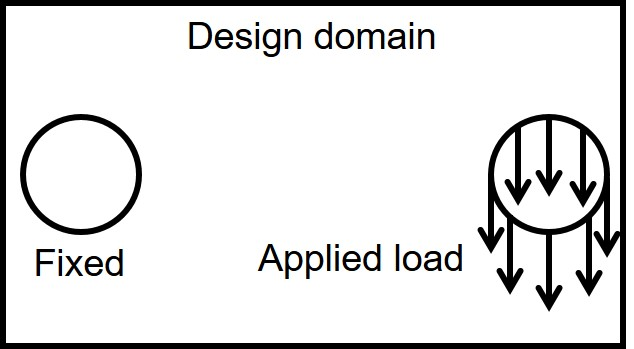
\includegraphics[width=0.5\textwidth]{domain.jpg}
\caption[Computational domain for the topology optimization]{Computational domain for the topology optimization} \label{fig:infill_domain}
\end{figure}


\begin{figure}[h]
\centering
\medskip
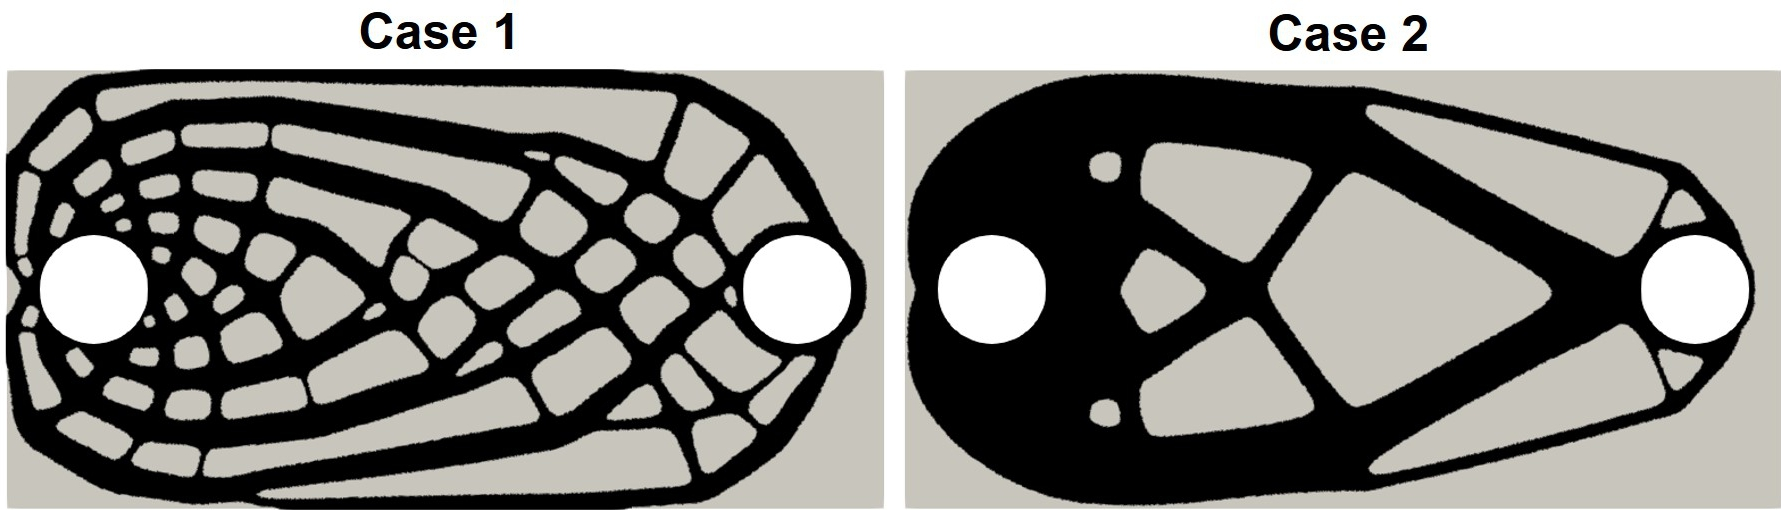
\includegraphics[width=\textwidth]{final_cases.jpg}
\caption[Topology optimization output to be used in the biodegradation simulations]{Topology optimization output to be used in the biodegradation simulations} \label{fig:infill_final_cases}
\end{figure}


\begin{figure}[h]
\centering
\medskip
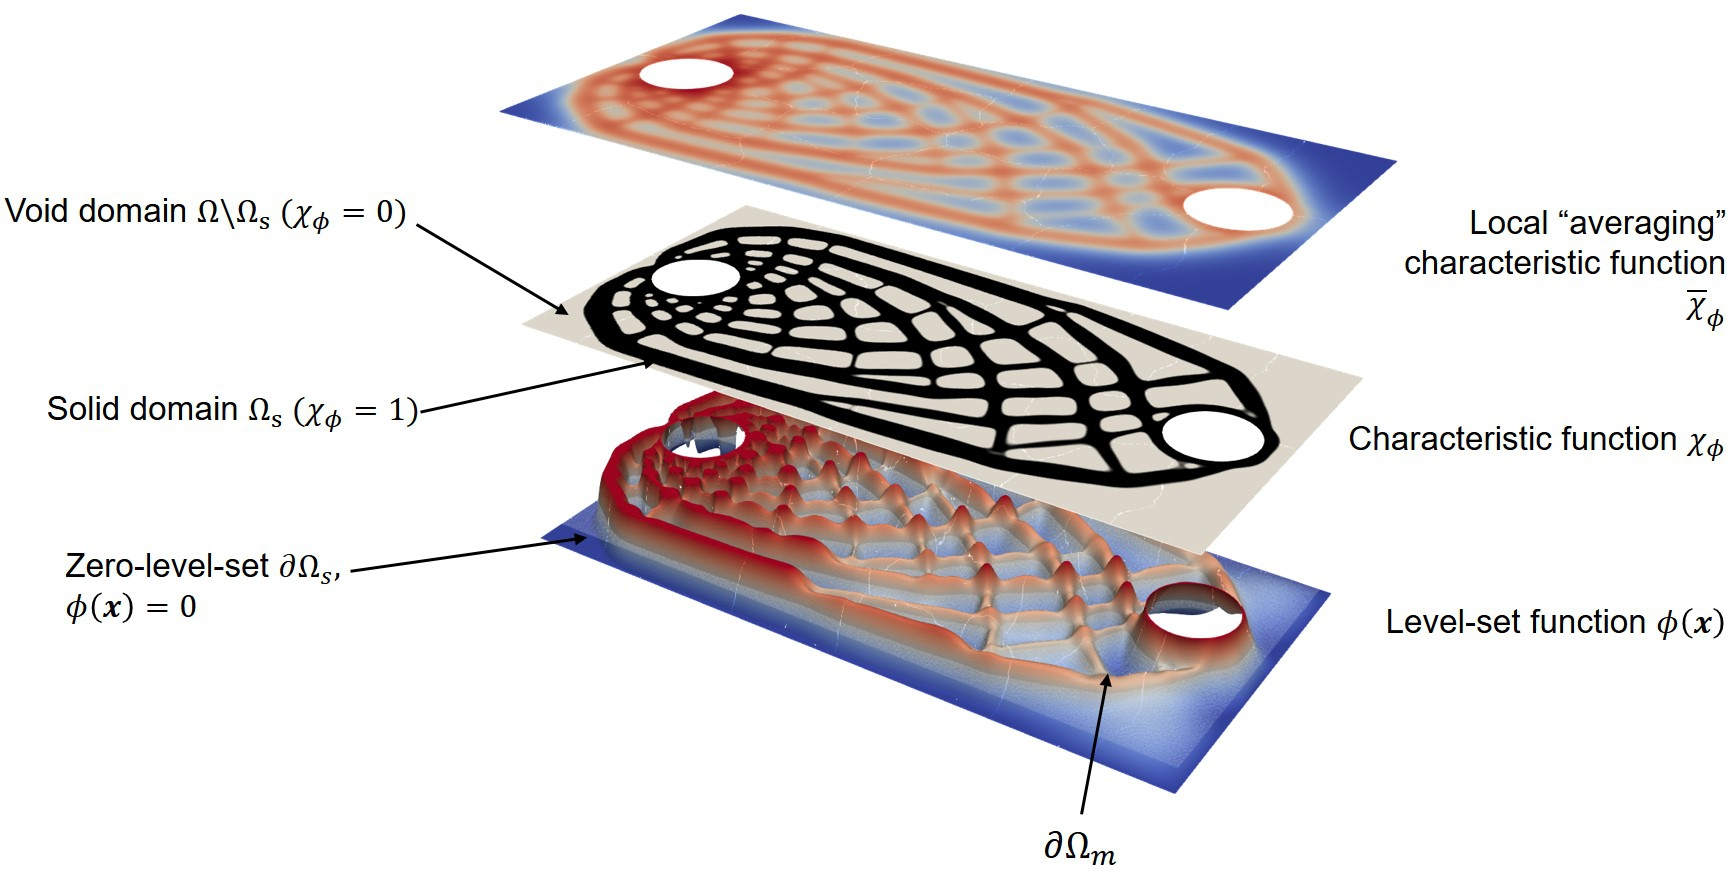
\includegraphics[width=\textwidth]{diagram.jpg}
\caption[Coupling topology optimization and biodegradation models]{Coupling topology optimization and biodegradation models} \label{fig:infill_diagram}
\end{figure}


\begin{figure}[h]
\centering
\medskip
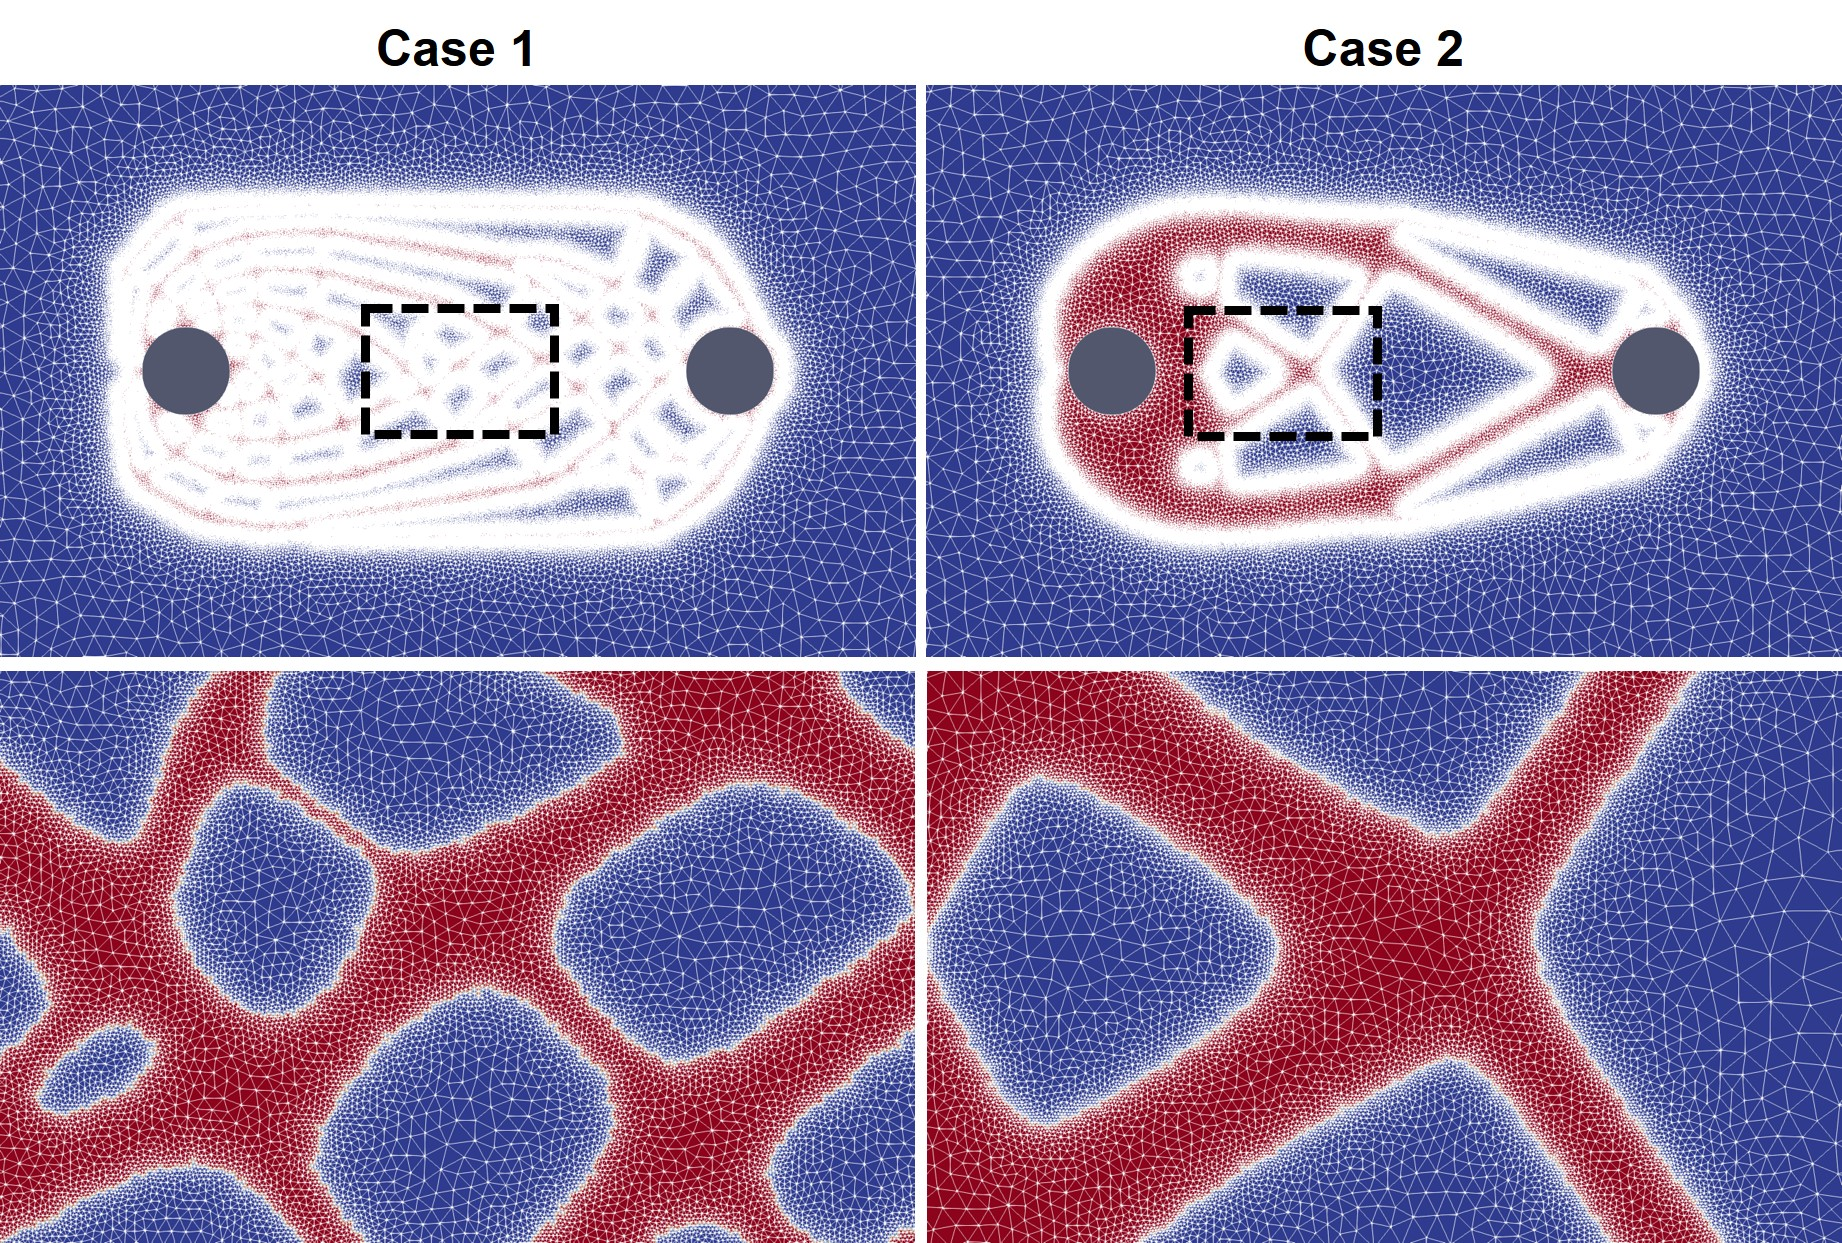
\includegraphics[width=\textwidth]{mesh.jpg}
\caption[Computational mesh for the biodegradation simulations]{Computational mesh for the biodegradation simulations} \label{fig:infill_mesh}
\end{figure}



\section{Results and Discussion}

The coupled biodegradation and structural mechanics models were constructed using the output of the TO procedure. Fig. \ref{fig:infill_case1_to_steps} shows the temporary evolving shapes of the infill during the optimization process for case 1, each of which is taken by skipping 40 intermediate steps. Fig. \ref{fig:infill_case2_to_steps} shows a similar 2D visualization for case 2.


\begin{figure}[h]
\centering
\medskip
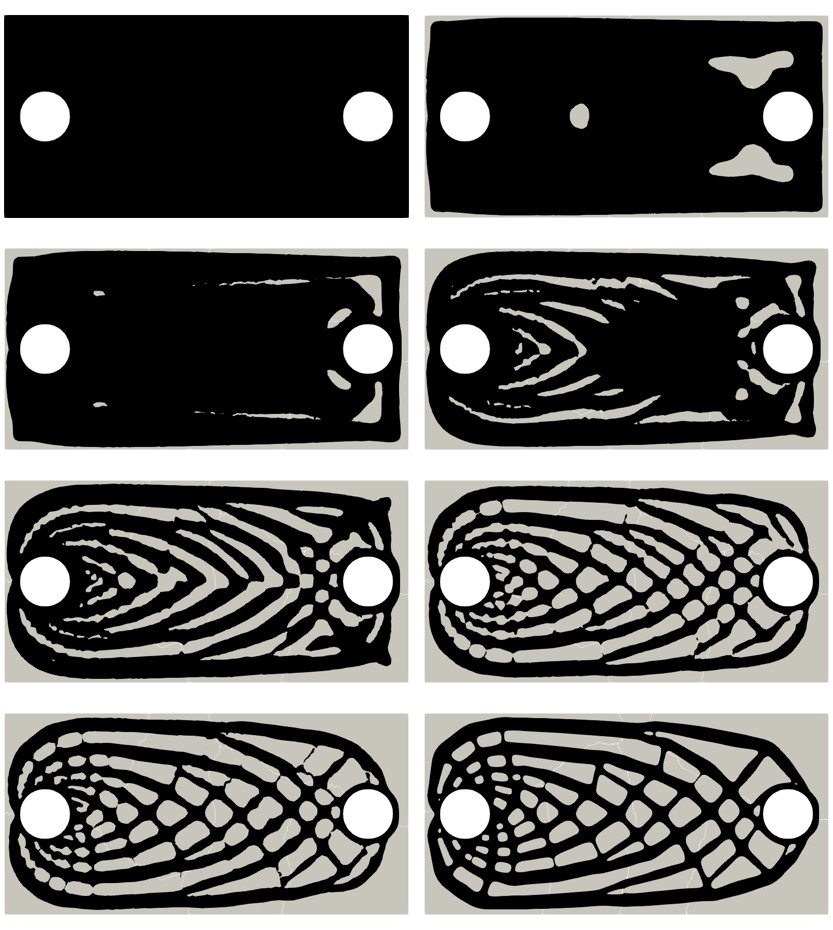
\includegraphics[width=\textwidth]{case1_to_steps.jpg}
\caption[Evolution of the topology optimization level set function for case 1]{Evolution of the topology optimization level set function to get the optimized shape for case 1, in which a local volume constraint was imposed.} \label{fig:infill_case1_to_steps}
\end{figure}

\begin{figure}[h]
\centering
\medskip
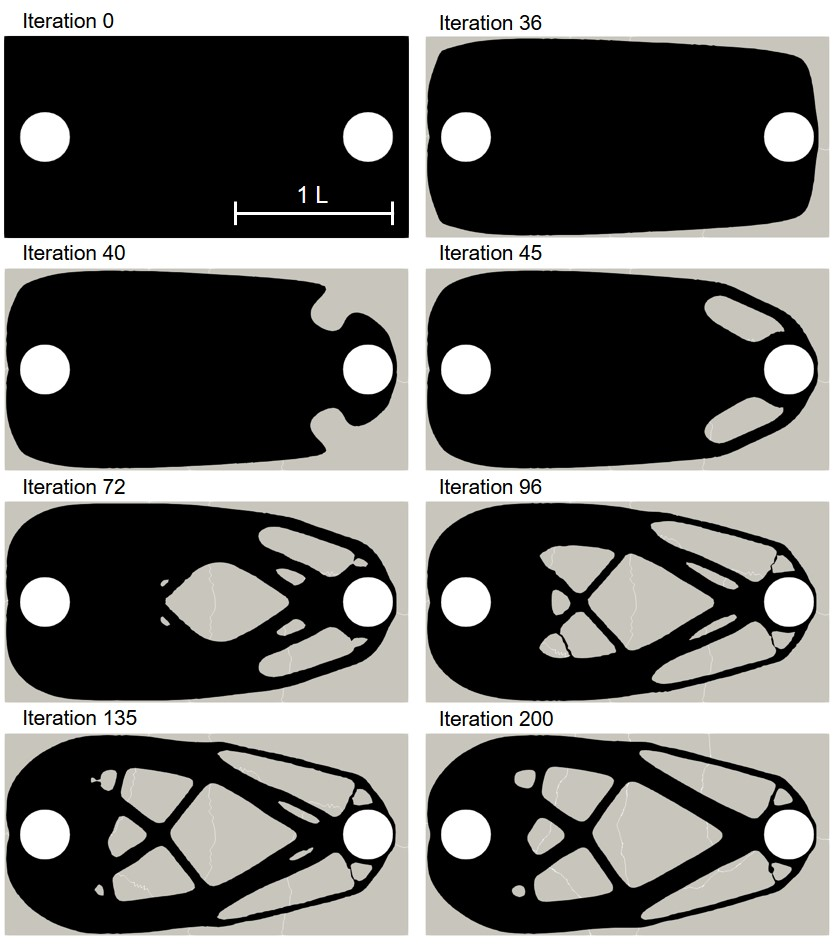
\includegraphics[width=\textwidth]{case2_to_steps.jpg}
\caption[Evolution of the topology optimization level set function for case 2]{Evolution of the topology optimization level set function to get the optimized shape for case 1, where only the global volume constraint was imposed.} \label{fig:infill_case2_to_steps}
\end{figure}

Fig. \ref{fig:infill_degradation_stiffness} shows the quantitative results of both components of the coupled computational model for the investigated cases. On the top row, the degradation rate is plotted by measuring the mass loss over time, showing how the diffusion rate of the Mg ions affects the rate of biodegradation in this model. On the bottom row, the change of the stiffness during the biodegradation is plotted, where the stiffness is calculated by inverting the compliance, the objective function of the TO routine calculated in each time step after adjusting the geometry in presence of degradation.


\begin{figure}[h]
\centering
\medskip
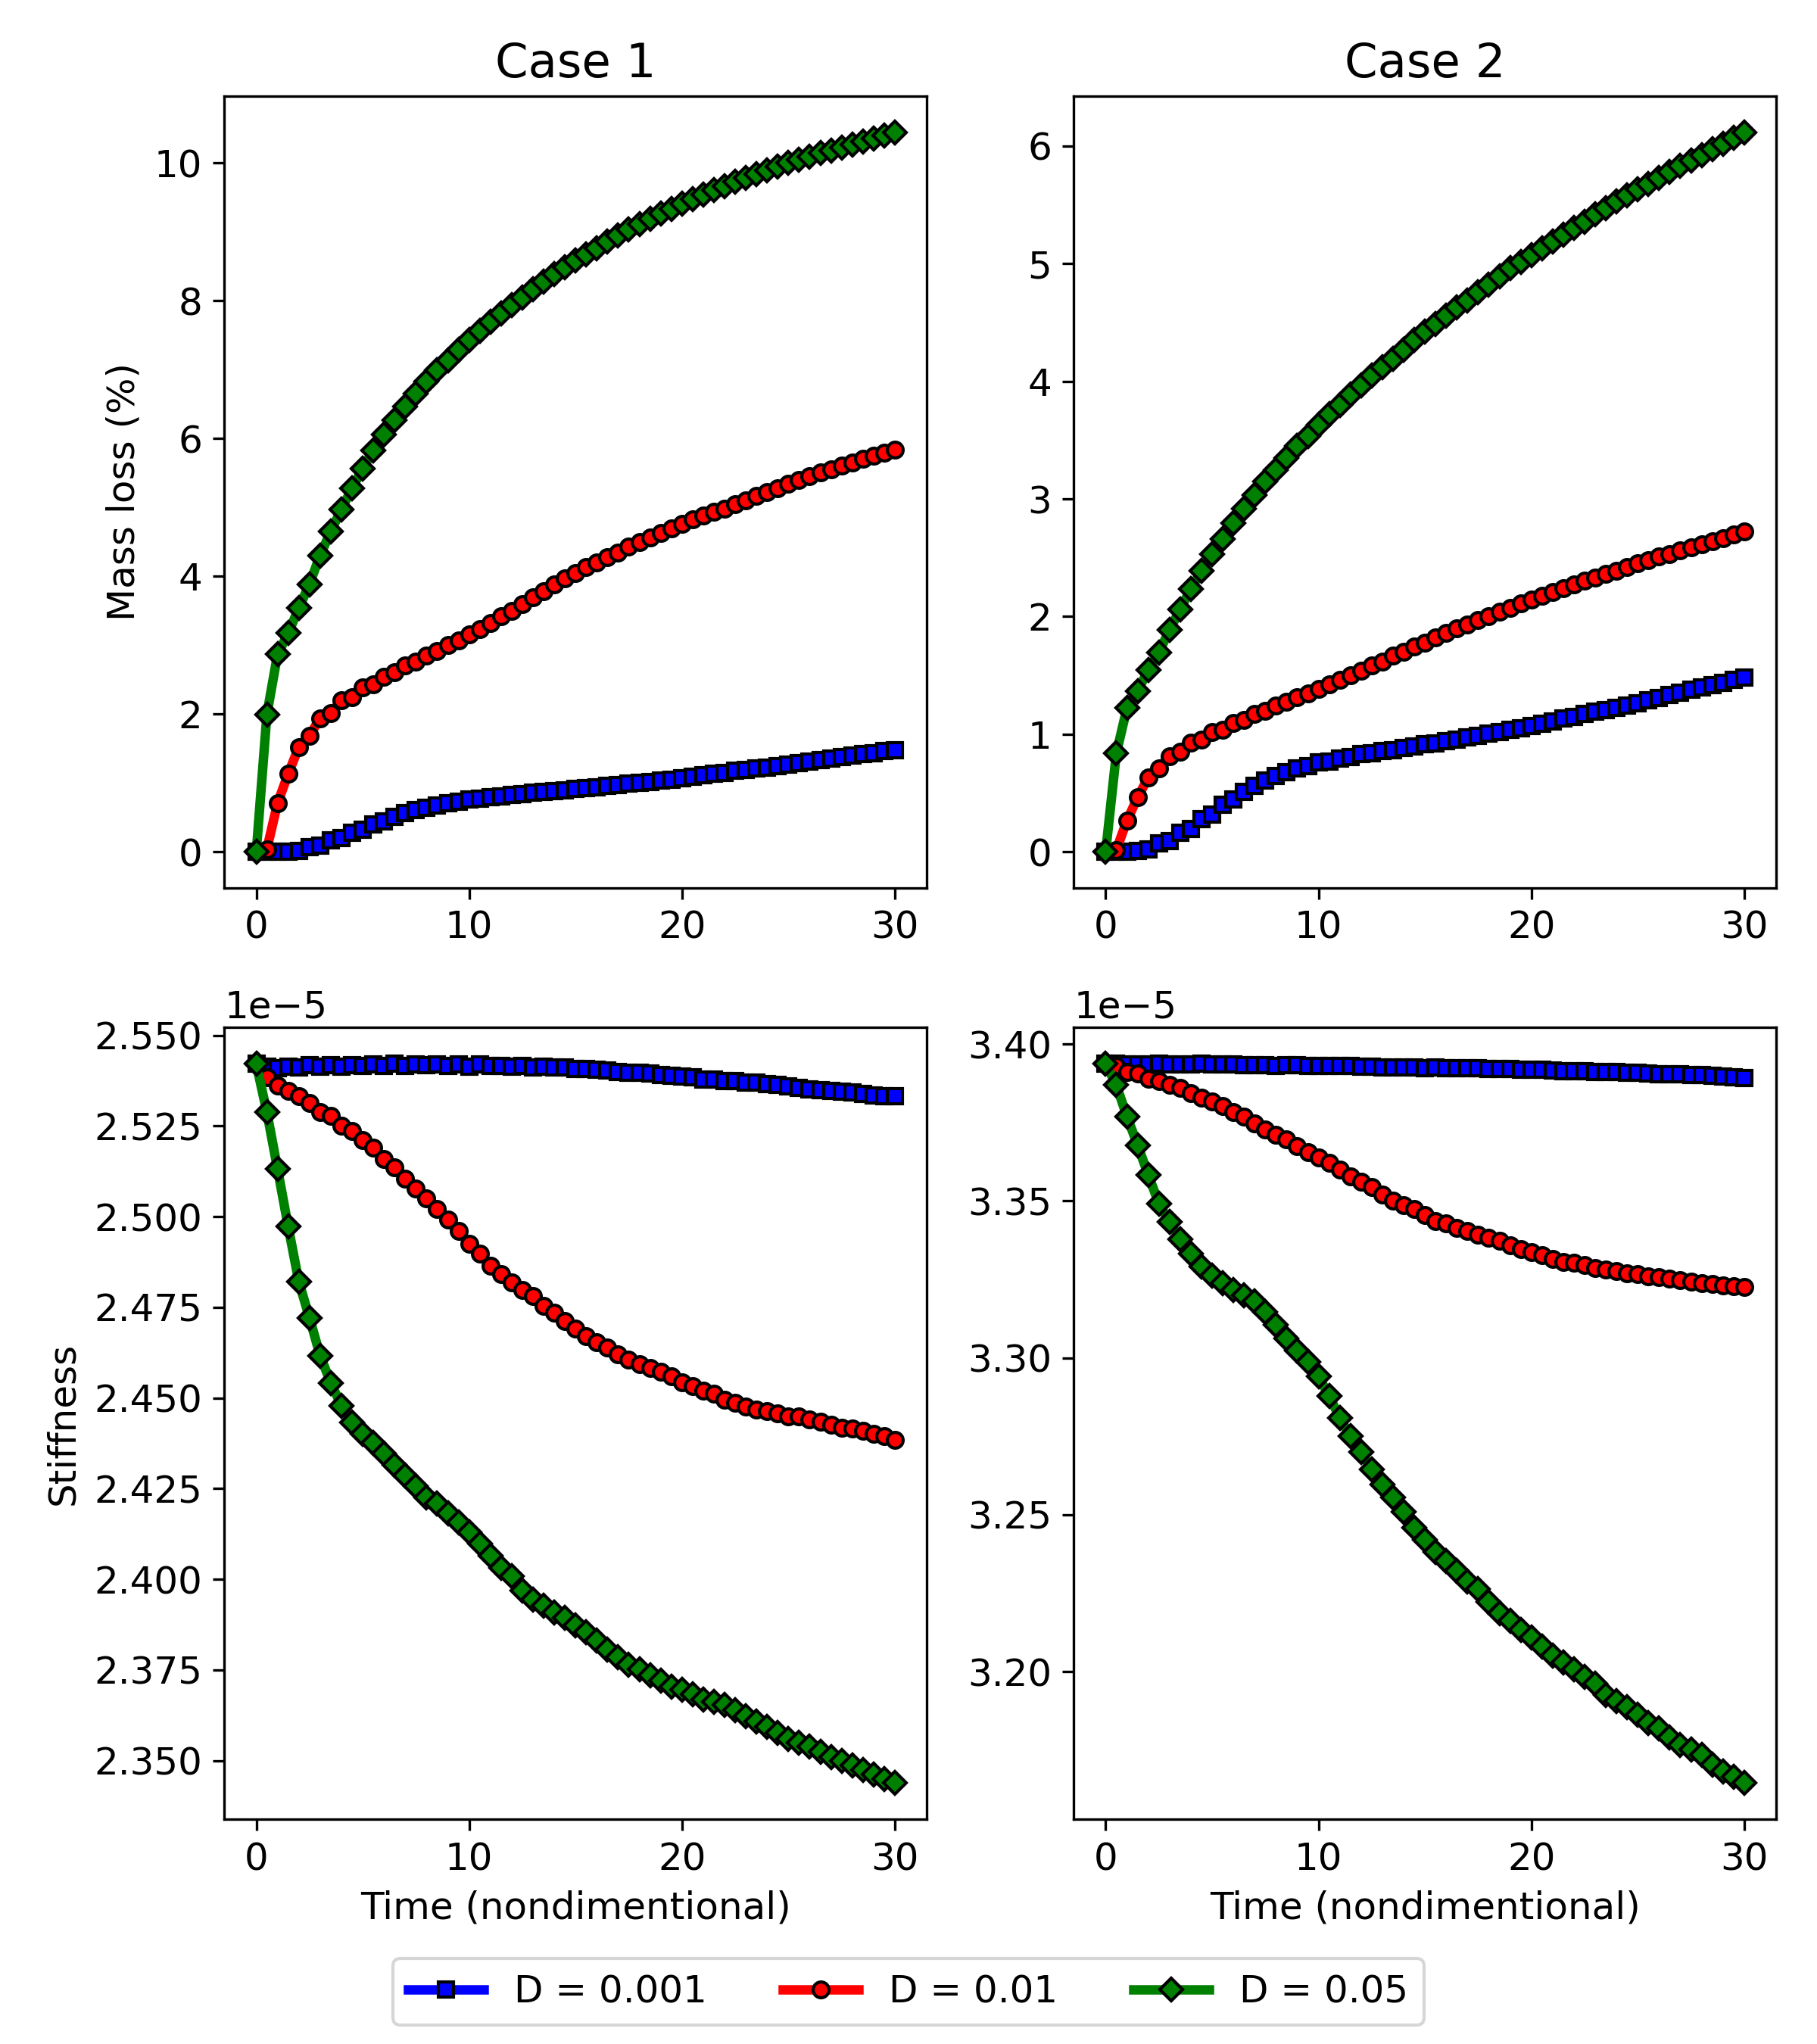
\includegraphics[width=\textwidth]{degradation_stiffness.png}
\caption[Results of the coupled model to predict the stiffness changes during biodegradation]{Results of the coupled model to predict the mass loss and stiffness changes during the biodegradation process of the infilled shapes.} \label{fig:infill_degradation_stiffness}
\end{figure}

Fig. \ref{fig:infill_results_mechanics} demonstrate how the qualitative results of the coupled model look like, in which the infilled part goes under the degradation and mechanical load at the same time. The green surface is the result of the mechanical analysis, visualized by bending the part according to the computed deformation vector in each node. The light green surface is the degradation object without bending being visualized, showing the change of the morphology due to biodegradation while the release of the metallic ions are also depicted.


\begin{figure}[h]
\centering
\medskip
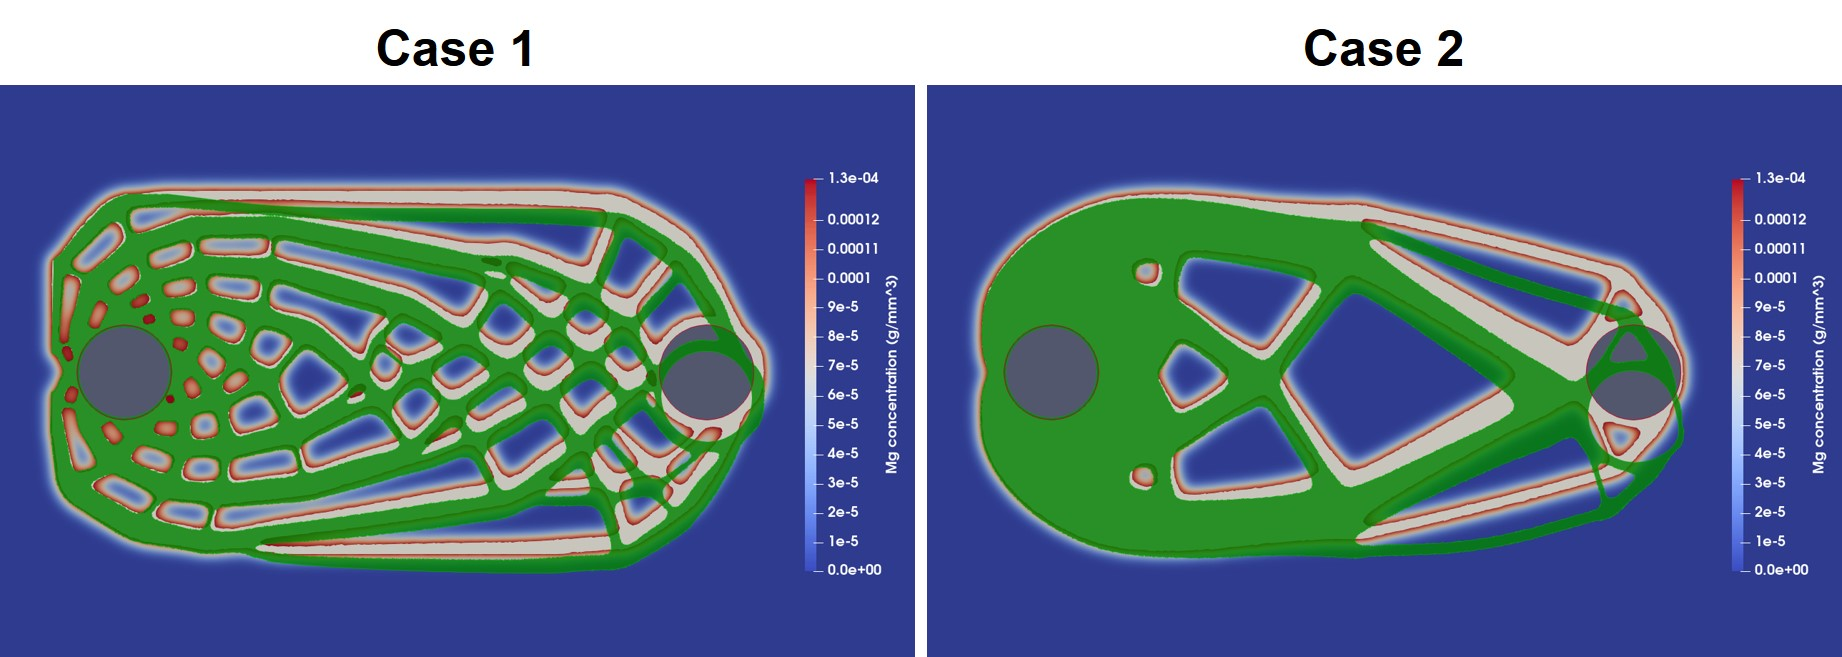
\includegraphics[width=\textwidth]{results_mechanics.jpg}
\caption[Coupled model results showing the stiffness analysis taking place during biodegradation simulation]{Coupled model results showing the stiffness analysis taking place during the biodegradation simulation. The green surface shows the deformed infilled structure, and the light gray surface is the state of the morphology during biodegradation. The colors show the concentration of metallic ions as being released from the surface of the degrading part.} \label{fig:infill_results_mechanics}
\end{figure}

In order to visualize the biodegradation only, the green surface is removed from Fig. \ref{fig:infill_results_mechanics}, and the results are plotted in various time points during the process. Figs. \ref{fig:infill_results_degradation_case1} and \ref{fig:infill_results_degradation_case2} show such visualization for case 1 and case 2, respectively, in which the surface of the degrading part is depicted in light gray, showing how the metallic ions are released during the biodegradation process. 

\begin{figure}[h]
\centering
\medskip
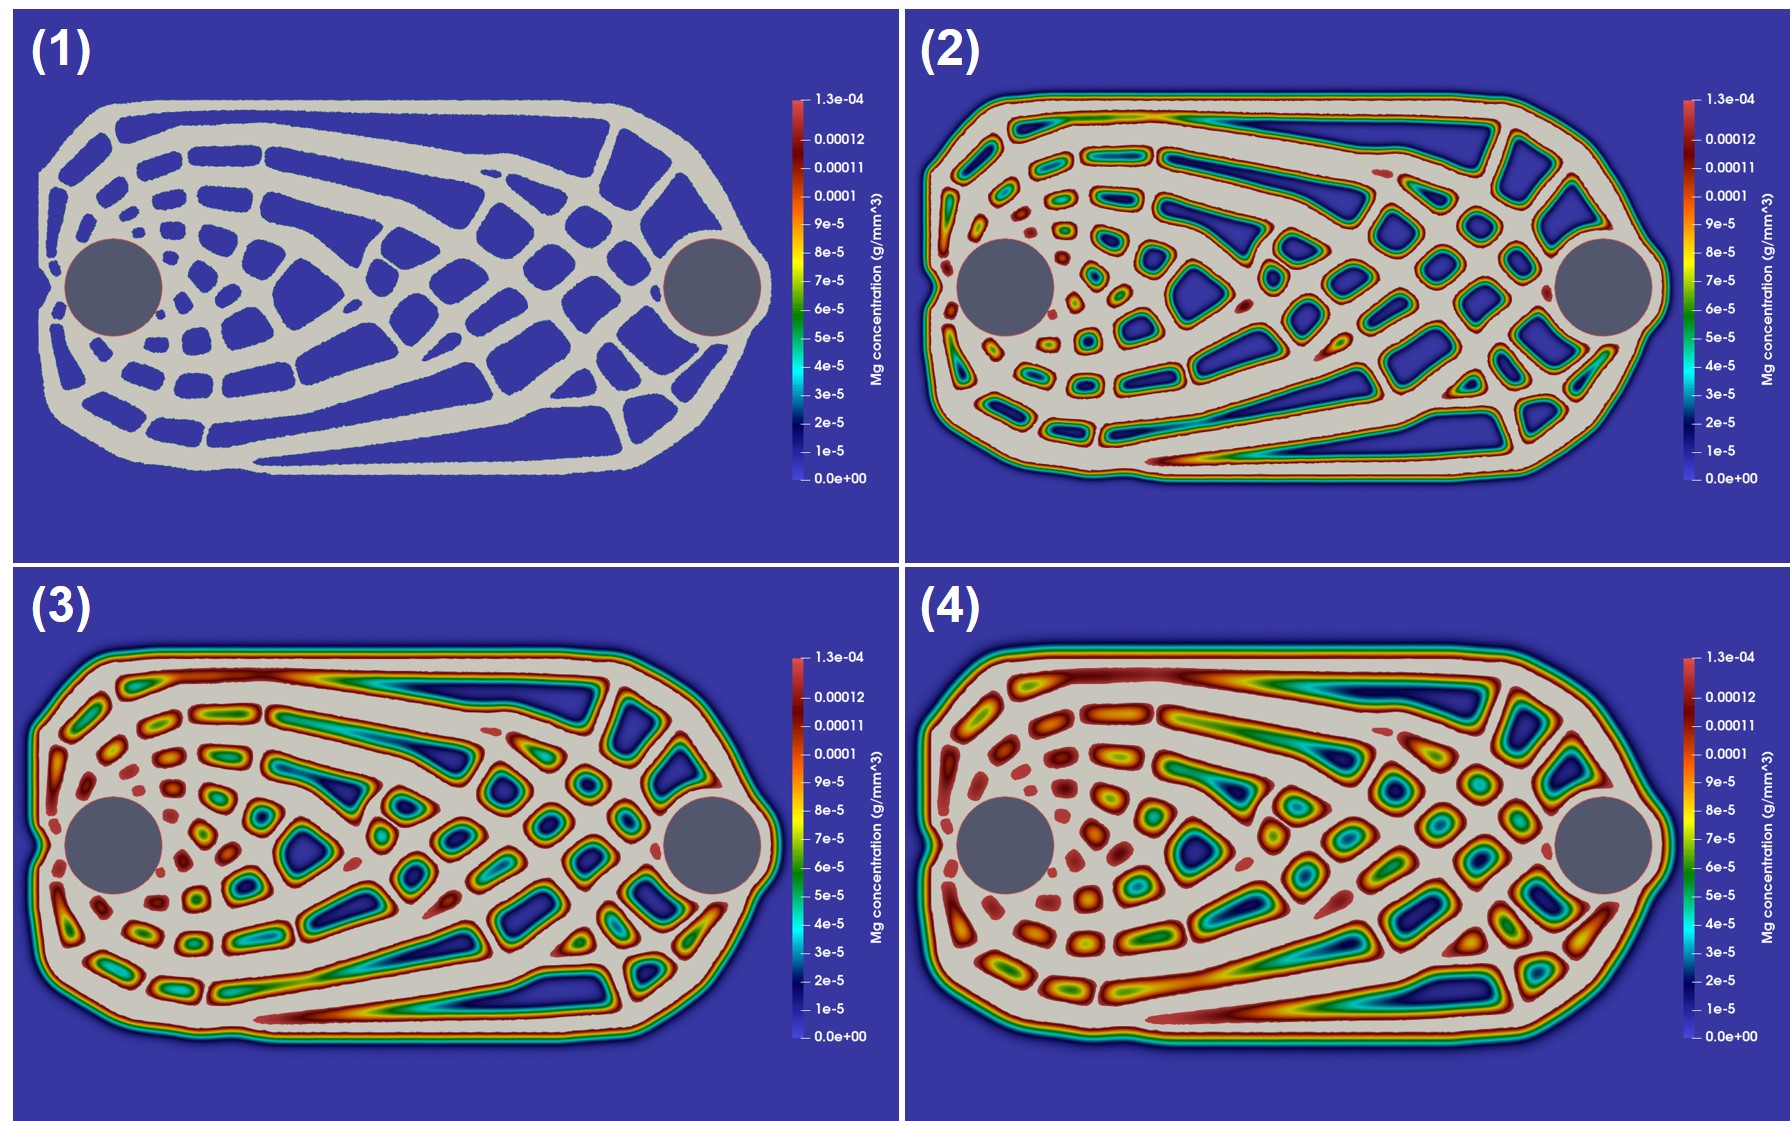
\includegraphics[width=\textwidth]{results_degradation_case1.jpg}
\caption[Visualization of the results of the biodegradation simulation for case 1]{Visualization of the results of the biodegradation simulation for case 1, showing the degrading of the infilled structure and release of Mg ions over time. The colors depict the Mg ions concentration.} \label{fig:infill_results_degradation_case1}
\end{figure}


\begin{figure}[h]
\centering
\medskip
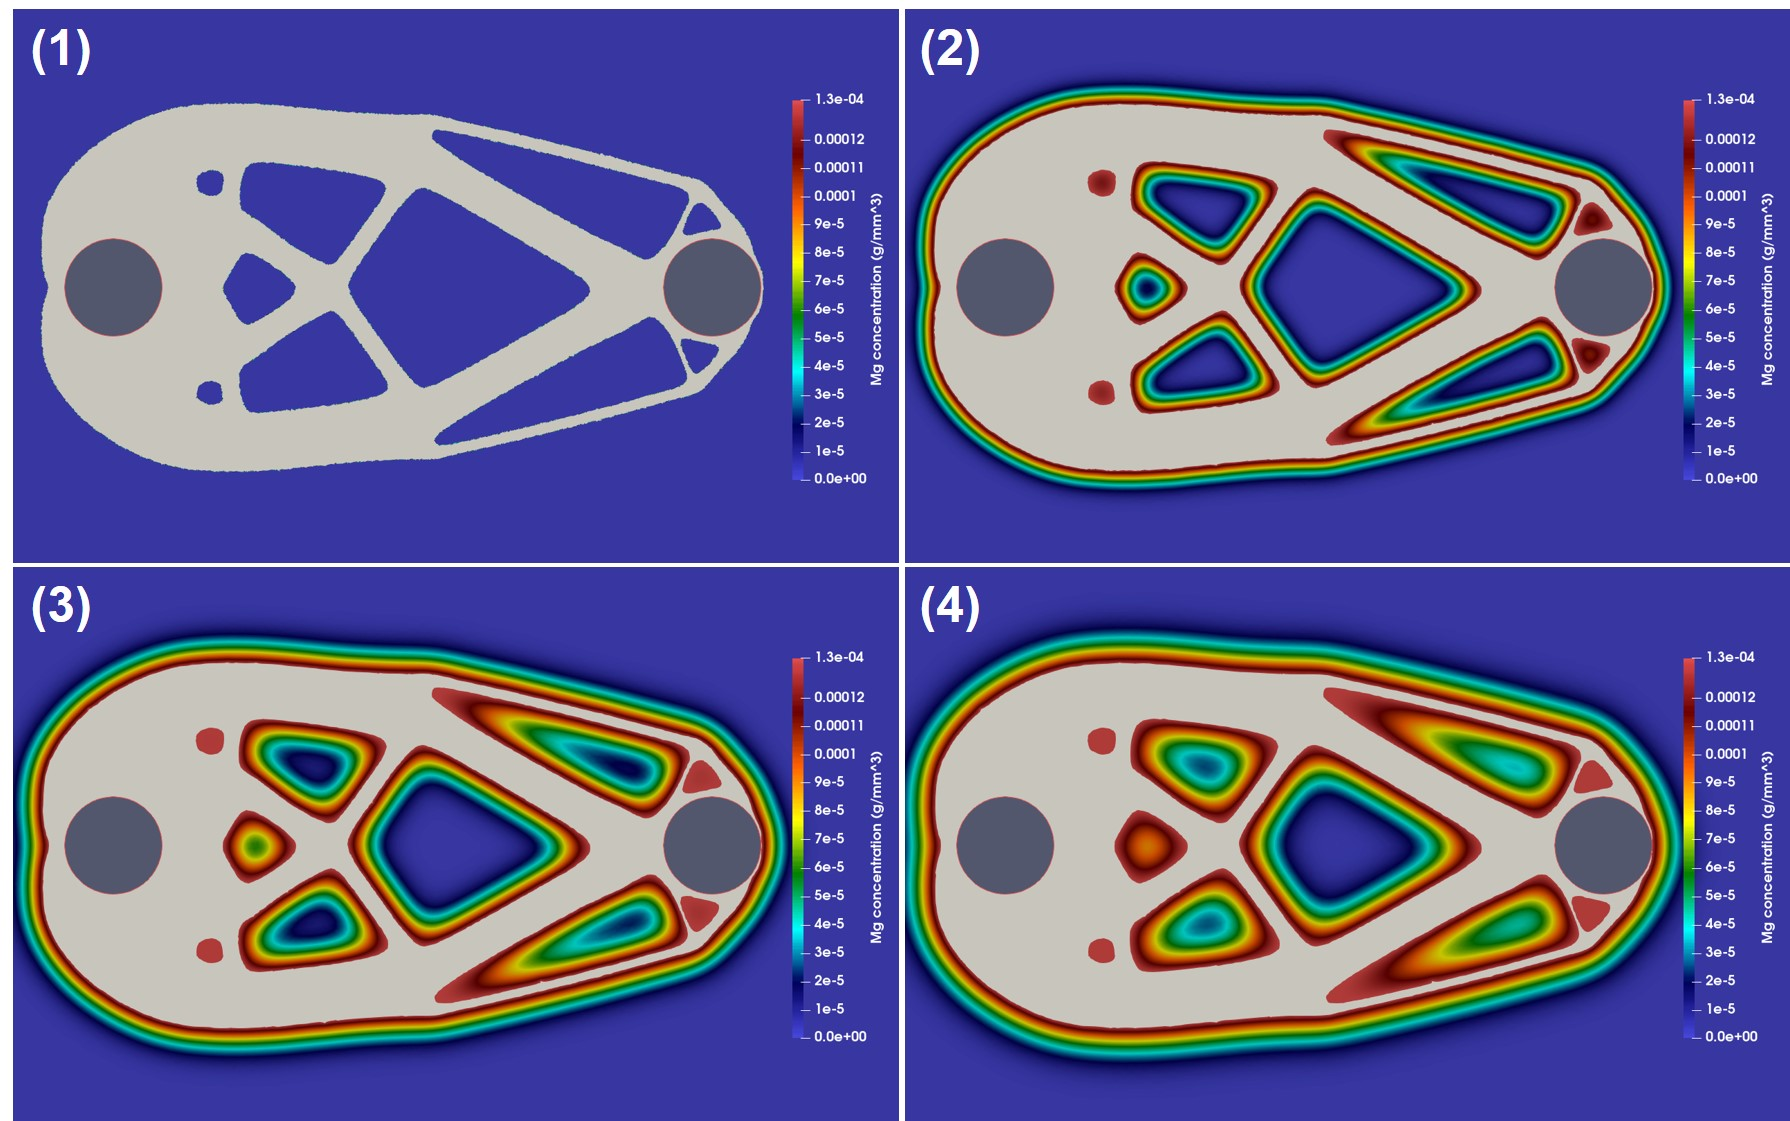
\includegraphics[width=\textwidth]{results_degradation_case2.jpg}
\caption[Visualization of the results of the biodegradation simulation for case 2]{Visualization of the results of the biodegradation simulation for case 2, showing the degrading of the infilled structure and release of Mg ions over time. The colors depict the Mg ions concentration.} \label{fig:infill_results_degradation_case2}
\end{figure}

As mentioned before, in order to increase the accuracy of the employed interface capturing method, the biodegradation model needs a refined mesh on the metal-environment interface. A closer look at the results of Fig. \ref{fig:infill_results_degradation_case1}, depicted in Fig. \ref{fig:infill_results_degradation_case1_zoom}, shows the mesh being refined on the interface. In this figure, the colors show the concentration of Mg ions released from the interface, and the biodegradation can be observed by the shrinkage of the light gray surface representing the undegraded parts of the infilled object.


\begin{figure}[h]
\centering
\medskip
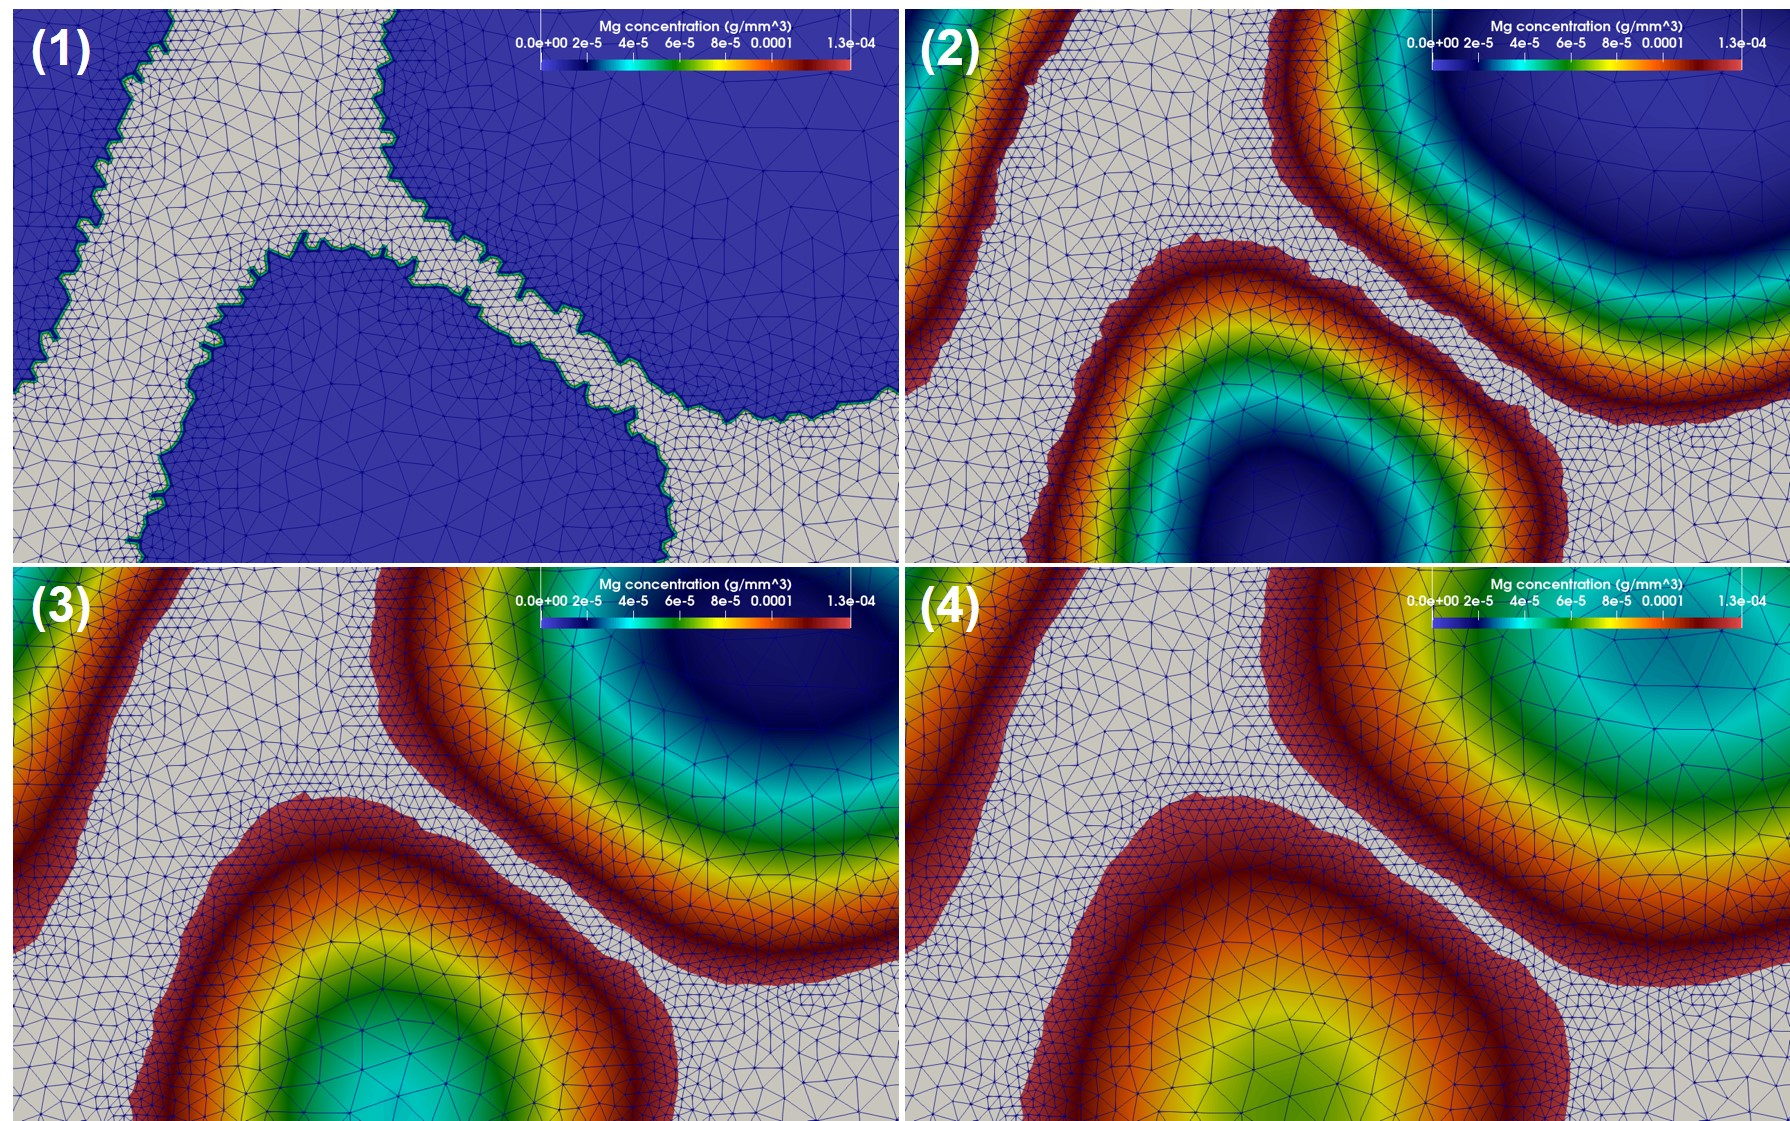
\includegraphics[width=\textwidth]{results_degradation_case1_zoom.jpg}
\caption[Zoom view of the results of the biodegradation simulation for case 1]{Zoomed view of the visualization results of the biodegradation simulation for case 1, showing the refined mesh, concentration of released ions, and shrinkage of the degrading object.} \label{fig:infill_results_degradation_case1_zoom}
\end{figure}

%%%%%%%%%%%%%%%%%%%%%%%%%%%%%%%%%%%%%%%%%%%%%%%%%%
% Keep the following \cleardoublepage at the end of this file, 
% otherwise \includeonly includes empty pages.
\cleardoublepage

